\section{Theory of \tmsn}~\label{sec:theory}

We start with a general description of loss-based learning. This
description can apply to both supervised and unsupervised learning.

We denote a model by $M$ and a data point by $\vx$. The datapoints are
generated by a fixed but unknown distribution $\Dist$. A model 


a randomly selected datapoint
by $\vx$\footnote{The \tmsn\ framework can be applied to both
  supervised and unsupervised learning.} and the loss associated with
model $M$ applied to the example $\vx$ by $L(M,\vx)$. Using this
notation 
$\vec{x}$ 
To streamline our presentation
we consider binary classification, but other supervised or
unsupervised learning problem can be accommodated with little change.

We are given
\newcommand{\cD}{{\cal D}}
\begin{itemize}
\item A set of classifiers $\strongRules$, each classifier $H \in
  \strongRules$ is a mapping from an input space $X$ to a binary label $\{-1,+1\}$.
\item A stream of labeled examples $(x_1,y_1),(x_2,y_2),\ldots$, $x_i
  \in X$, $y_i \in \{-1,+1\}$, generated IID according to a fixed but
  unknown distribution $\cD$.
\end{itemize}

The goal of the algorithm is to find a classifier $H \in
\strongRules$ that minimized the error probability $\err(H)\doteq
P_{(x,y) \sim \cD}[H(x) \neq y]$

All workers start from the same initial classifier $H_0$ which is
improved iteratively. Some iterations end with the worker finding a
better classifier by itself, others end with the worker receiving a
better classifier from another worker. The sequences of classifiers
corresponding to different workers can be different, but with high
probability they all converge to the same classifier.

Denote each worker by an index $i=1,\ldots,n$. On iteration $t$
each worker has its {\em current} classifier  $H_i(t)$ and a set of $m$
{\em candidate} classifiers $G_i^j(t)$. An error upper bound
$\errub(H_i(t))$ is associated with $H_i(t)$ so that with high
probability $\errub(H_i(t)) \geq \err(H_i(t))$.

\begin{figure}[t]
\begin{center}
  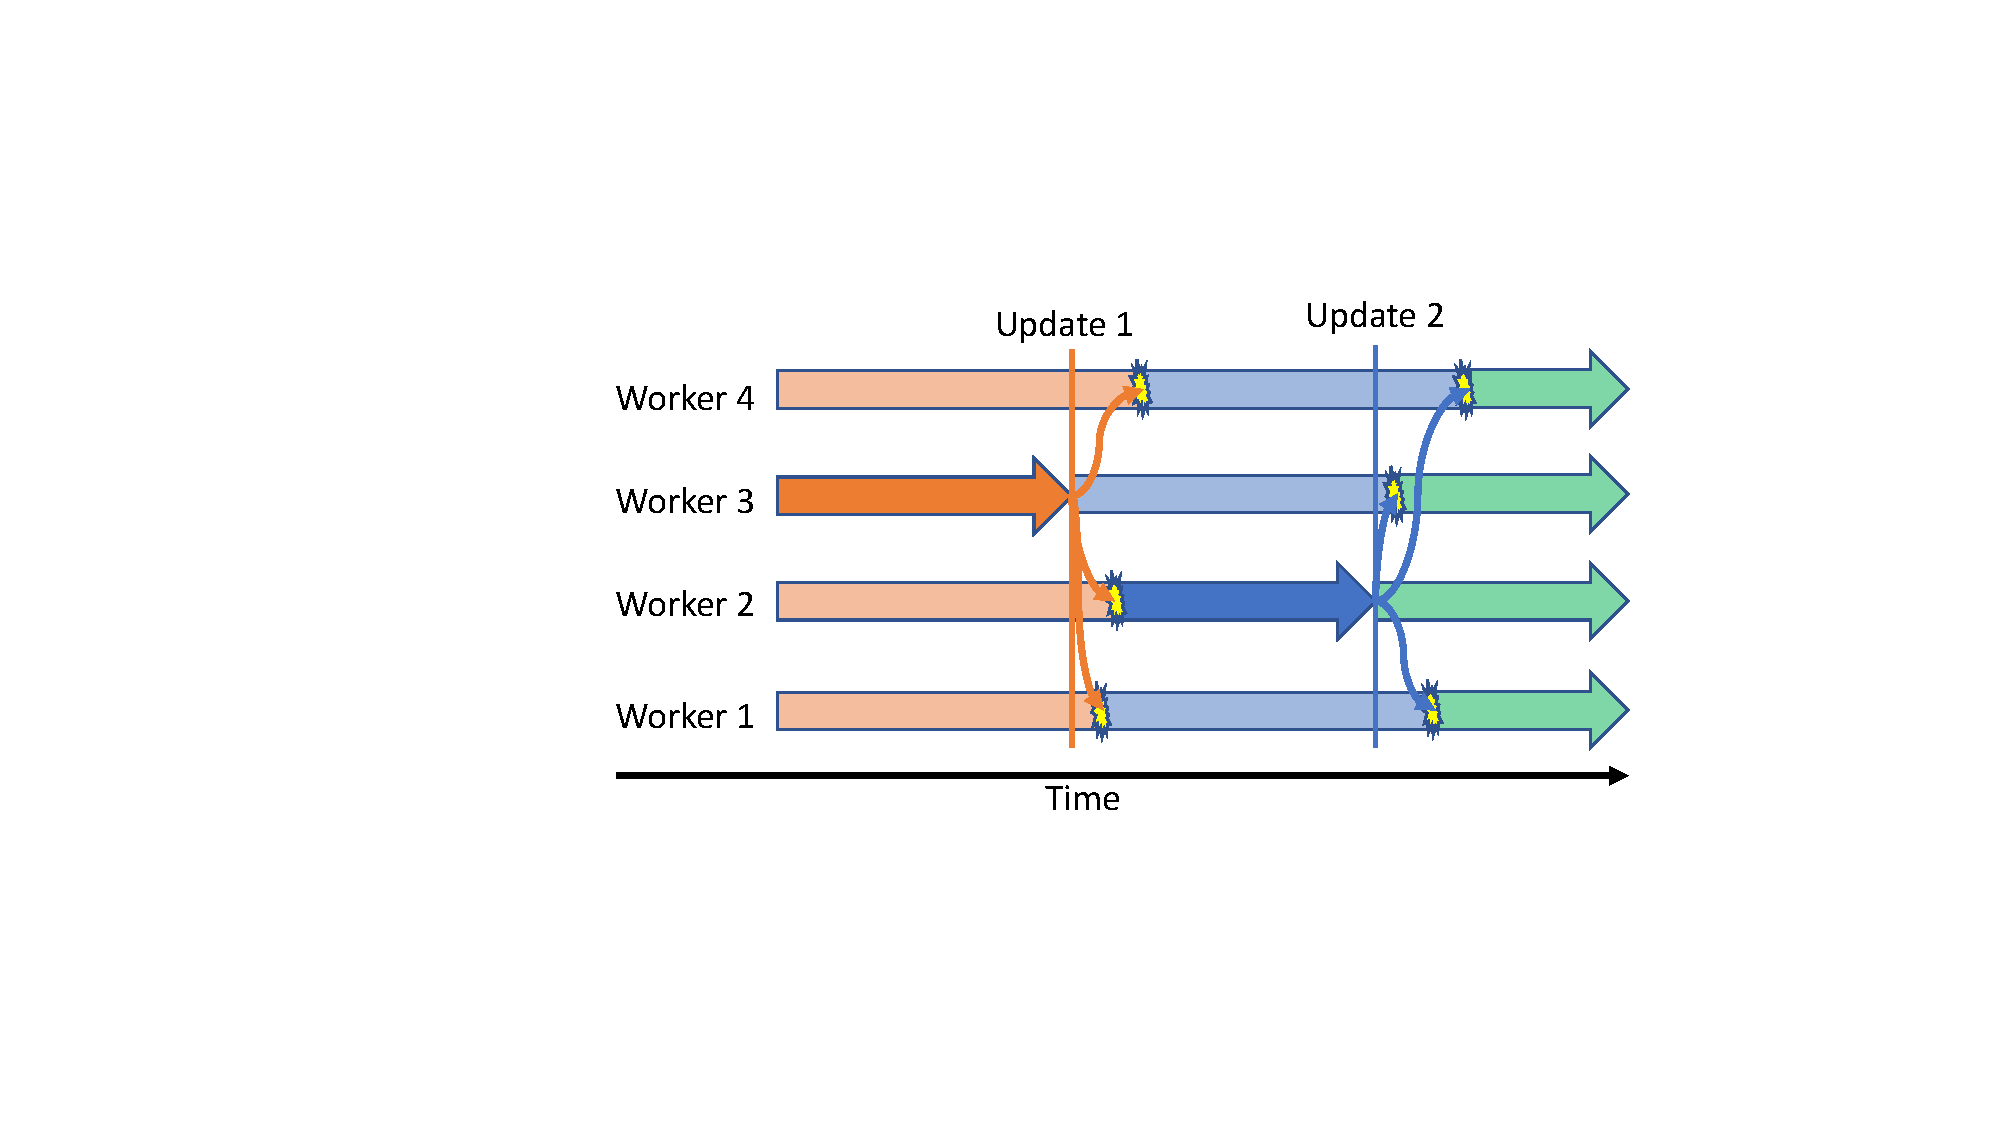
\includegraphics[width=0.5\textwidth]{AsyncUpdates.pdf}
\end{center}
  \caption{{\bf Execution timeline of a \tmsn\ system}
      System consists of four workers. The first update occurs when
      worker 3 identifies a better classifier $H_1$. It then replaces
      $H_0$ with $H_1$ and broadcasts $(H_1,z_1)$ to the
    other workers. The other workers receive the message the at different
    times, depending on network congestion. At that time they  interrupt the
    scanner (yellow explosions) and start using $H_1$. Next, worker 2
    identifies an improved rule $H_2$ and the same process ensues.
    \label{fig:async}}
   	\vspace{0pt}
%\end{minipage}
\end{figure}

The worker reads examples from the stream and uses them to estimate
the errors of the candidates. It stops when it finds a candidate that,
with high probability, has an error smaller than
$\errub(H_i(t))-\epsilon$ for some constant ``gap'' parameter
$\epsilon>0$.

More precisely, the worker uses a {\em stopping rule} that chooses a
stopping time and a candidate rule and has the property that, with
high probability, the chosen candidate rule has an error smaller than
$\errub(H_i(t))-\epsilon$. This candidate then replaces the current
classifier, the new upper bound is set to be $\errub(H_i(t+1)) =
\errub(H_i(t))-\epsilon$, a new set of candidates is chosen and the
worker proceeds to the next iteration. At the same time the worker
{\em broadcasts} the pair $(H_i(t+1), \errub(H_i(t+1))$.

A separate process in each worker listens to broadcasts of this
type. When worker $i$ receives a pair $(H,\errub(H))$ it compares the
upper bound $\errub(H)$ with the upper bound associated with it's
current classifier $\errub(h_i(t))$. If $\errub(H) < \errub(h_i(t))-\epsilon$,
it interrupts the current search and sets $H_i(t+1)=H$. If not the
received pair is discarded.

Note that the only assumption that the workers make regarding the
incoming messages is that the upper bound $\errub(H)$ is sound. In
other words that, with hight probability, it is an upper bound on the
true error $\err(H)$. There is no synchronization and if a worker is
slow or fails, the effect on the other workers is minimal.

Different implementations of \tmsn\ differ in the way that they
generate candidate classifiers and in the stopping rules that they
use. For \tmsn\ to be effective, the stopping rule should be both
sound and tight. If it is not sound, then the scheme falls apart, and
if it is not tight, then the stopping rules stop later than needed,
slowing down convergence.

Next, we describe how \tmsn\ is applied to boosting.






\section{\tmsn\ for Boosting}~\label{sec:boost}
Boosting algorithms~\cite{schapire_boosting:_2012} are iterative, they generate a
sequence of {\em strong rules} of increasing accuracy. The strong rule
at iteration $T$ is a weighted majority over $T$ of the the weak rules
in $\cH$.
$$H_T(x) = \sign \left( \sum_{t=1}^T \alpha_t h_t(x) \right)$$

For the purpose of \tmsn\ we define $\strongRules$ to be the set of
strong rules combining any number of weak rules from $\cH$.

Boosting algorithms can be interpreted as gradient descent
algorithm~\cite{mason_boosting_1999}. Specifically, if we define the {\em potential} of
the strong rule $H$ with respect to the training set $\training$ to be
\[
\Z(H_T) \doteq \frac{1}{n} \sum_{i=1}^n e^{- y_i H_T(x_i)},
\]
then AdaBoost is equivalent to coordinate-wise gradient descent,
where the coordinates are the elements of $\cH$. Suppose we have the
strong rule $H$ and consider changing it to $H+\alpha h$ for some $h
\in \cH$ and for some small $\alpha$. The derivative of the potential
wrt $\alpha$ is:
$$
\left.\frac{\partial}{\partial \alpha}\right|_{\alpha=0} \Z(H+\alpha h) =
\frac{1}{n} \sum_{i=1}^n \left.\frac{\partial}{\partial \alpha}\right|_{\alpha=0} e^{ - y_i (H(x_i)+\alpha h(x_i))}
=
\frac{1}{n} \sum_{i=1}^n -y_i h(x_i) e^{- y_i H(x_i)}
$$
Our goal is to minimize the average potential $\Z(H_{T+1})$, therefor our goal is to
find a weak rule $h$ that makes the gradient negative. Another way of
expressing this goal is to find a weak rule with a large empirical {\em edge}:
\begin{equation} \label{eqn:gamma_emp}
\edgeEmp(h) \doteq  \sum_{i=1}^n w_i y_i h(x_i) \mbox{ where } w_i =
\frac{1}{Z}e^{- y_i H(x_i)}; Z = \sum_{i=1}^n e^{- y_i H(x_i)}
\end{equation}
$w_i$ defines a distribution over the training examples, with respect
to which we are measuring the correlation between $h(x_i)$ and $y_i$.
This is the original view of boosting, which is the
process of finding weak rules with significant edges with respect to
different distributions. We distinguish between the empirical
edge $\edgeEmp(h)$, which depends on the sample, and the {\bf true} edge, which
depends on the underlying distribution:
\begin{equation} \label{eqn:gamma_emp}
\edge(h) \doteq E_{(x,y) \sim \Dist}( w(x,y) y h(x)) \mbox{ where }
w(x,y)=\frac{1}{Z} \Dist(x,y) e^{- y H(x)}
\end{equation}
and $Z$ is the normalization factor with respect the the true
distribution $\Dist$.

A small but important observation is that boosting does not require
finding the weak rule with the {\bf largest} edge at each
iteration. Rather, it is enough to find a rule for which we are sure
that it has a significant (but not necessarily maximal)
advantage. More precisely, we want to know that, with high probability
over the choice of $\training \sim \Dist^n$  the rule $h$ has a significant
{\em true} edge $\edge(h)$.

\paragraph{Sequential Analysis and Early Stopping}\label{sec:methods:early-stop}
The standard approach when looking for the best weak rule
is to compute the error of candidate rules using
all available data, and then select the rule $h$ that maximizes the empirical
edge $\edgeEmp(h)$. However, as described above, this can be
over-kill. Observe that if the true edge $\edge(h)$ is large it can be
identified as such using a small number of examples.

Bradley and Schapire~\cite{bradley_filterboost:_2007} and Domingo and
Watanabe~\cite{domingo_scaling_2000} proposed using early stopping to
take advantage of such situations. The idea is simple: instead of
scanning through all of the training examples when searching for the
next weak rule, a {\em stopping rule} is checked for each $h \in \cH$
after each training example, and if this stopping rule ``fires'' then
the scan is terminated and the $h$ that caused the rule to fire is
added to the strong rule. We use early stopping in our algorithm.

For reasons that will be explained in the next section, we use a different
stopping rule than~\cite{bradley_filterboost:_2007}
or~\cite{domingo_scaling_2000}. We use a stopping rule proposed
in~\cite{balsubramani_sharp_2014} for which they prove the following

\begin{theorem}[based on \cite{balsubramani_sharp_2014} Theorem 4] \label{thm:balsubramani}
  Let $M_t$ be a martingale $M_t = \sum_i^t X_i$,
  and suppose there are constants $\{c_k\}_{k \geq 1}$ such that
  for all $i \geq 1$, $|X_i| \leq c_i$ w.p.\ 1.
  For $\forall \sigma > 0$, with probability at least $1 - \sigma$ we have
  \[
  \forall t: |M_t| \leq C \sqrt{
    \left( \sum_{i=1}^t c_i^2 \right)
    \left( \log \log \left( \frac{ \sum_{i=1}^t c_i^2 }{ |M_t| }\right) +
    \log \frac{1}{\sigma} \right)
  },
  \]
  where $C$ is a universal constant.
\end{theorem}

\paragraph{Effective Sample Size}
\label{sec:effectiveSampleSize}
Equation~\ref{eqn:gamma_emp} defines $\edgeEmp(h)$, which is an
estimate of $\edge(h)$. How accurate is this estimate? Our initial
gut reaction is that if $\training$ contains $n$ examples the error should be
about $1/\sqrt{n}$. However, when the examples are weighted this is
clearly wrong. Suppose, for example that $k$ out of the $n$ examples
have weight one and the rest have weight zero. Obviously in this case
we cannot hope for an error smaller than $1/\sqrt{k}$.

A more quantitative analysis follows. Suppose that the weights of the
examples in the training set $\training=\{ (x_1, y_1), \ldots, (x_n,
y_n) \}$ are $w_1=w(x_1,y_1),\ldots,w_n=w(x_n,y_n)$. Thinking of
finding a good weak rule in terms of hypothesis testing, the null
hypothesis is that the weak rule $h$ has no edge. Finding a rule that
is significantly better than random corresponds to rejecting the
hypothesis that $\edge(h)=0$.  Assuming the null hypothesis, $y_i
h(x_i)$ is $+1$ with probability 1/2 and $-1$ with probability
$1/2$. From central limit theorem and assuming $n$ is larger than
$100$, we get that the null distribution for $\edgeEmp(h)=\sum_{i=1}^n
w_i y_i h(x_i)$ is normal with zero mean and standard deviation
$\sum_{i=1}^n w_i^2$. The statistical test one would use in this case
is the $\Ztest$-test for
\begin{equation} \label{eqn:Ztest}
\Ztest = \frac{\edgeEmp(h)}{\sqrt{\sum_{i=1}^n w_i^2}}
= \frac{\sum_{i=1}^n w_i y_i h(x_i)}{\sqrt{\sum_{i=1}^n w_i^2}}
\end{equation}
As should be expected, the value of $\Ztest$ remains the same whether
or not $\sum_{i=1}^n w_i=1$. Based on Equation~\ref{eqn:Ztest} we
define the {\em effective number of examples} corresponding to the
un-normalized weights $w_1,\ldots,w_n$ as:
\begin{equation} \label{eqn:neff}
  \neff \doteq \frac{\left(\sum_{i=1}^n w_i\right)^2}{\sum_{i=1}^n w_i^2}
\end{equation}
Owen~\cite{owen_monte_2013} used a different line of
argument to arrived at a similar measure of
the effective samples size for a weighted sample.

The quantity $\neff$ plays a similar role in large deviation bounds
such as the Hoeffding bound~\cite{hoeffding_probability_1963} (details ommitted).
It also plays
a central role in Theorem~\ref{thm:balsubramani} and thus in the
stopping rule that we use.

To understand the important role that $\neff$ plays in our algorithm,
supppose the training set is of size $n$ and that only $m \ll n$
examples can fit in memory. Our approach is to start by placing a
random subset of size $m$ into memory and then run multiple
boosting iterations using this subset. As the strong rule improves,
$\neff$ decreases and as a result the stopping rule based on
Theorem~\ref{thm:balsubramani} requires increasingly more examples
before it is triggered. When $\neff/m$ crosses a pre-specified
threshold the algorithm flushes out the training examples currently in
memory and samples a new set of $m$ examples using acceptance
probability proportional to their weights. The new examples have
uniform weights and therefor after sampling $\neff=m$.

Intuitively, weighted sampling utilizes the computer's memory better
than uniform sampling because it places in memory more difficult
examples and fewer easy examples. The result is better estimates of
the edges of specialist\footnote{Specialist weak rules and their
  advantages are described in Section~{sec:Algorithm}} weak rules that
make predictions on high-weight difficult examples.


Another concern is the fraction of the examples that are selected. In
the method described here the expected fraction is $(\frac{1}{n}
\sum_{i=1}^n w_i)/(\max_i w_i)$.
